\section{Knowledge Graph Construction}\label{sec-kgconstruct}
Despite numerous well-established KGs~\cite{hoffart2013yago2, tian2023graph}, they treat nodes/edges as entities/relations, which necessitates sophisticated relational extraction techniques and thereby limits their applicability in general domains~\cite{huang2021knowledge}. Additionally, their primary focus on the Wikipedia domain also restricts their usage for answering non-Wikipedia questions such as ones over legal or financial documents. To remedy this issue, we propose generally applicable KG construction methods.


We first analyze two representative questions in Figure~\ref{fig-question}(a)-(b) to motivate our KG construction. Answering these two questions necessitates the deduction of logical associations among different passages. These associations are encoded either through 1) lexical similarity: common keywords shared among different passages, e.g., `Alf Clausen' bridges passage $\mathbf{S}_1$ and passage $\mathbf{S}_2$ in Figure~\ref{fig-question}(a), or 2) semantic similarity: syntactic elements that convey semantic relations, e.g., `nationality' and `American director' in Figure~\ref{fig-question}(b). This motivates us to construct the graph by modeling passages as nodes and their lexical/semantic similarity as edges. More specifically in Figure~\ref{fig-graphconstruct}, we split each document into individual passages, and for each passage $\mathbf{S}_i$, we add a node $v_i$ to the KG with its feature being the text of that passage $\mathcal{X}_i$. Then we add edges by checking the lexical/semantic similarity between pairs of passage nodes. 

\subsubsection{TF-IDF KG Construction} For adding edges according to lexical similarity, we first
% construct the nodes' bag-of-word (BOW) features. Instead of considering words from every document, we 
apply TF-IDF keyword extraction~\cite{ramos2003using} over each document to filter out meaningless words such as supporting verbs and articles, which also reduces the dimension of bag-of-word (BOW) features, sparsifies the constructed graph and increases the graph traversal efficiency. In addition, we add the document title into the extracted keyword set since some questions focus on title entities. We collect the extracted keywords from all documents to form the keyword space $\mathcal{W}$ and then connect two passages if they share any common keyword in $\mathcal{W}$.

% We collect all extracted keywords to form the keyword space $\mathcal{W} = \{w_i\}_{i = 1}^{|\mathcal{W}|}$ with $|\mathcal{W}|$ being its cardinality and construct the BOW features $\mathbf{B}_i\in\{0, 1\}^{|W|}$ for each sentence $v_i \in \mathcal{V}$ where $\mathbf{B}_{ij} = 1$ indicates the $i^{\text{th}}$ sentence has the $j^{\text{th}}$ keyword and $\mathbf{B}_{ij} = 0$ otherwise. Then we connect two sentences if they share common keywords.
% Note that nodes' BOW features $\mathbf{X}$ are different from nodes' textual features $\mathcal{X}$. The former one is a binary matrix while the latter one is textual sentences. Then if two nodes share any common keyword in $\mathcal{W}$, we add an edge between them.

\begin{figure*}[t!]
    \centering
    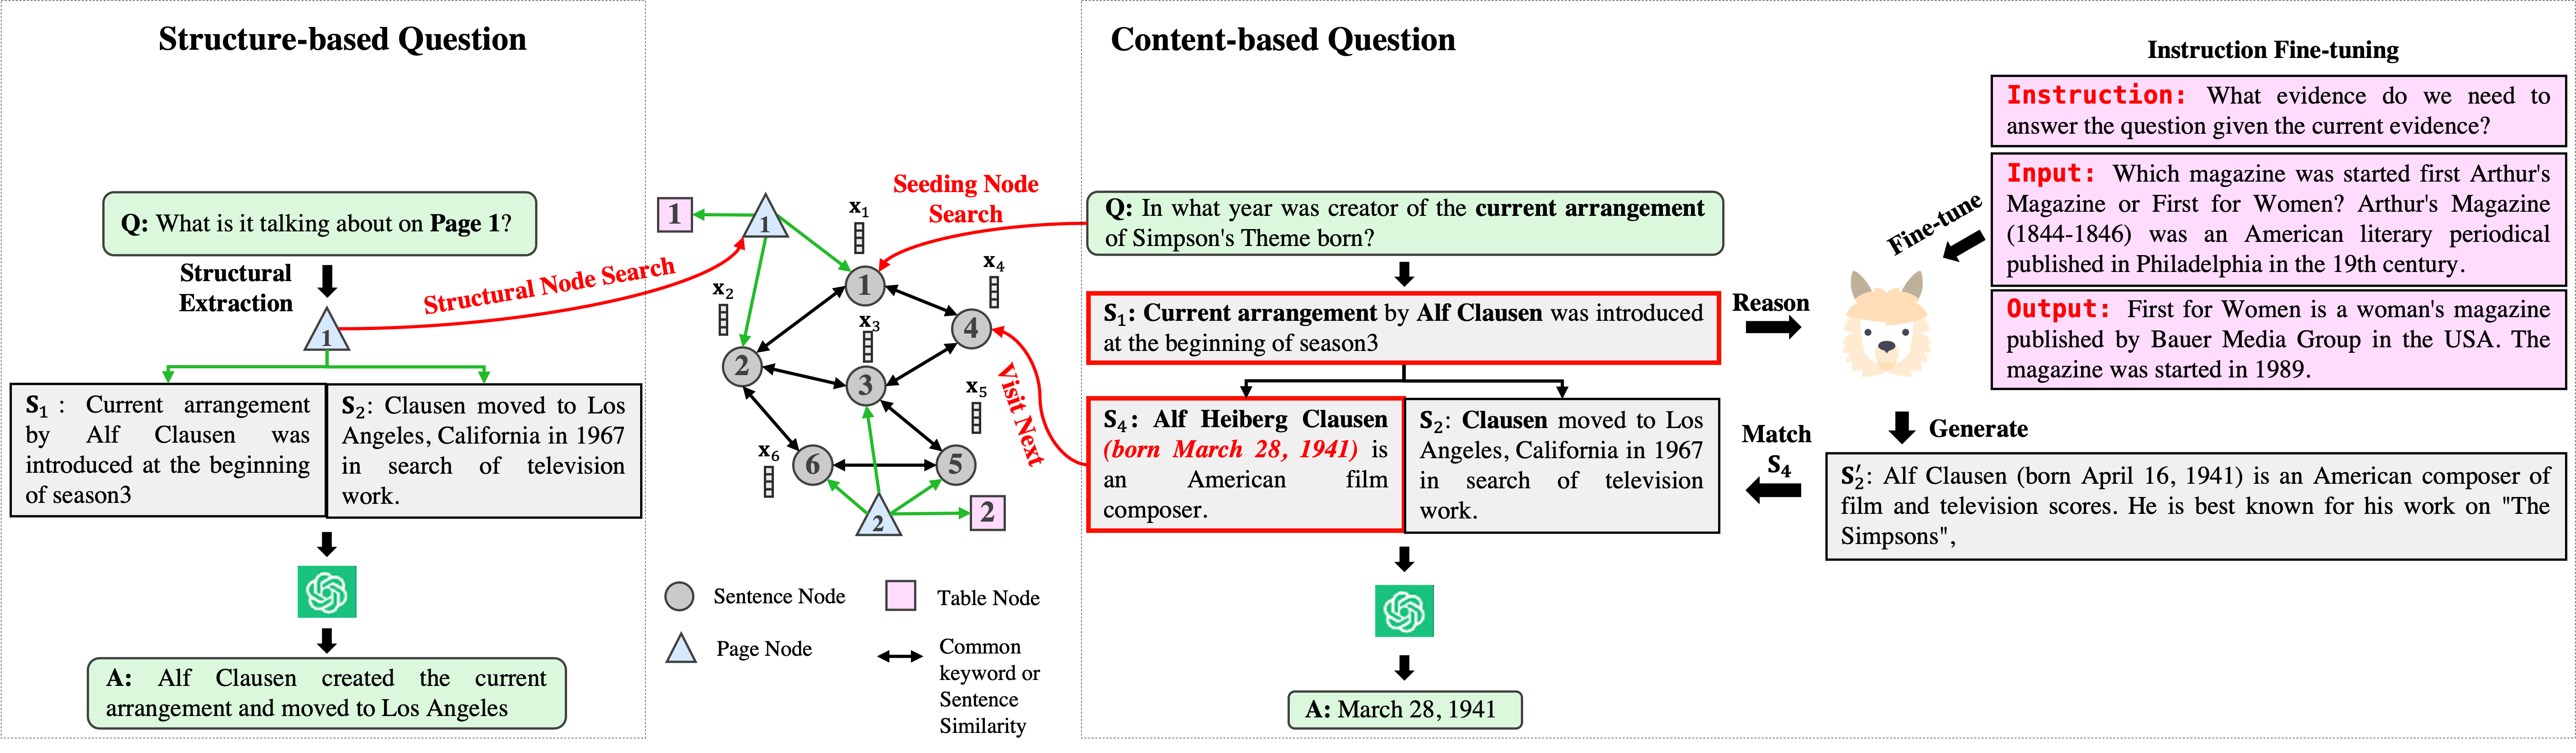
\includegraphics[width=\textwidth]{Figure/path_generator.png}
    \caption{LLM-based KG traversal agent for context retrieval. For questions on document structures (left), we employ LLM to extract structures and retrieve their corresponding contents (the content of pages are passages belonging to that page and the content of tables is the markdown-formatted text). For questions on document content, we concatenate it with the currently retrieved context and prompt the LLM to generate the next evidence to answer the question. By comparing the similarity between the candidate neighboring sentences and the generated passage, we determine the next passage node to traverse. Correspondingly, the candidate neighbors are updated for the next round of traversal.}
    \label{fig-graphwalker}
    \vspace{-2ex}
\end{figure*}

\subsubsection{KNN-ST/MDR KG Construction} For adding edges according to semantic similarity, we can readily employ pre-existing models such as sentence transformers to generate passage embedding $\mathbf{X}_i$ for each node $v_i$ and subsequently compute pairwise similarity matrix to construct the K-nearest neighbor (KNN)
graph. However, these off-the-shelf models, typically trained on tasks not so-related to MD-QA, may not adequately encapsulate necessary logical associations in their embedding similarity demanded by the question. To overcome this problem, we follow the training strategy of MDR~\cite{xiong2020answering} and train a sentence encoder by predicting the subsequent supporting facts based on previously supporting facts, thereby endowing the encoder with reasoning capability. Consequently, the embedding similarity and the corresponding constructed KNN graph fundamentally encapsulate the necessary logical associations between different passages. 

\subsubsection{TAGME} Moreover, we employ TAGME~\cite{min2019knowledge} to extract Wikipedia entities from each passage and construct the graph based on whether two passage nodes share common Wikipedia entities.


In addition to passage nodes, we further add structural nodes into the graph by extracting document structures via Extract-PDF~\footnote{\url{https://developer.adobe.com/document-services/docs/overview/pdf-extract-api/}}. In this paper, we only consider adding pages and tables but the constructed KG can include more different types of document structures. The feature of table nodes is the markdown since LLMs can understand this as demonstrated in Figure~\ref{fig-tableunderstanding} in Supplementary. The feature of page nodes is the page number and we add directed edges from it to sentence/table nodes in that page. \textit{Note that we do not aim to propose a one-size-fits-all KG construction method. Instead, we seek to compare the merits and limitations of various methods in Table~\ref{tab-compare}, offering guidance on which KGs are best suited for specific scenarios.}


\begin{figure}[t!]
    \hspace{-2ex}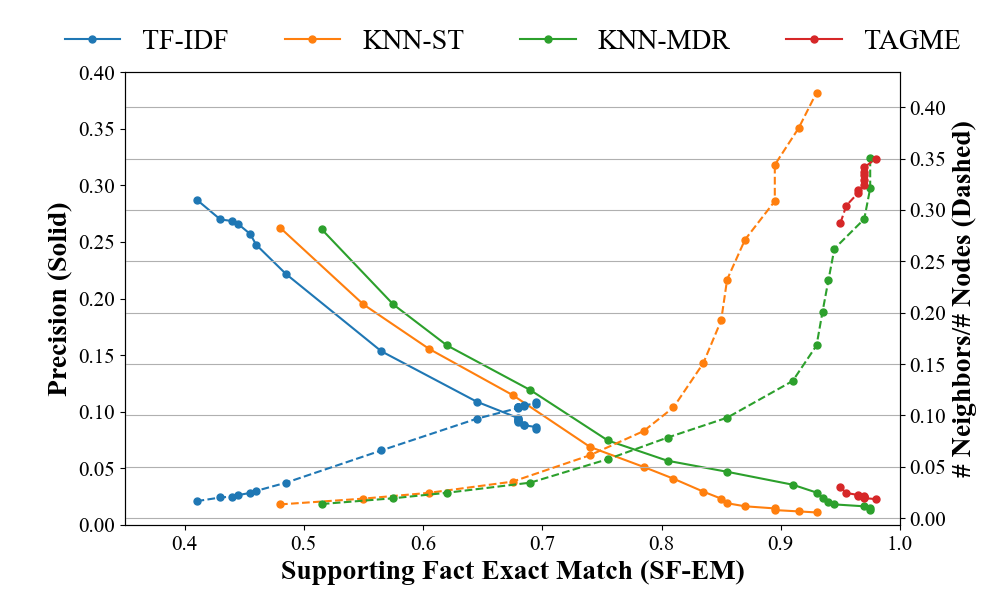
\includegraphics[width=0.5\textwidth]{Figure/hotpotqa_graph.png}
    \caption{Quality of KGs on HotpotQA. For each KG Construction method, as the average number of neighbors increases (KG becomes denser) in the right y-axis, the SF-EM increases while the precision decreases. KNN-MDR achieves a better trade-off than TF-IDF and KNN-ST. KGs constructed by TAGME are denser than others.}
    \label{fig-hotpotqa_graph}
    \vspace{-5ex}
\end{figure}


\newpage
To verify the constructed KGs indeed encode the necessary information for MD-QA, we randomly sample questions from HotpotQA and construct KGs over the set of documents for each of these questions using our proposed methods. We vary the hyperparameters to control the sparsity of the constructed KG and measure how much percentage of the supporting facts are covered by neighbors of the seeding passages initially searched by TF-IDF. More details about the four construction methods and their hyperparameters are included in Section~\ref{sup-KGC} in Supplementary. As shown in Figure~\ref{fig-hotpotqa_graph}, as the constructed graph becomes denser, the chance that the neighboring node passages hit the supporting facts increases (i.e., SF-EM increases) although the redundant information also increases (i.e., the precision decreases). Given the common keywords shared between one passage to all other passages are typically far less than the total number of passages across all documents, the density of the constructed graph by TF-IDF would be upper-bounded, causing lower SF-EM (evidenced by SF-EM below 0.7 in Figure~\ref{fig-hotpotqa_graph} for TF-IDF curve). For TAGME, we empirically find it identifies a larger quantity of entities mentioned in a single passage, which leads to a denser graph and causes the starting SF-EM of TAGME to be already around 0.95. In addition, since KNN-MDR is pre-trained by predicting the next supporting facts~\cite{xiong2020answering} on HotpotQA, it achieves better trade-off than KNN-ST where the embeddings are directly obtained from the sentence transformer without dataset-specific pre-training. 


To summarize, although high SF-EM indicates that the supporting facts for most questions are fully covered by the neighbors of seeding passages, low precision signifies that most of these neighboring passages are irrelevant to the question. Therefore, if we blindly perform graph traversal without any question-tailored adaptation, our retrieved contexts would include redundant passages and compromise the capability of LLMs in MD-QA (which is also verified by the lower performance of KGP-Random in Table~\ref{tab-ablation}). To remedy this issue, in the next section, we introduce an LLM-based KG traversal agent to adaptively visit neighboring passages that are most conducive to answering the given question.


\section{LLM-based KG Traversal Agent}\label{sec-graphwalker}
A natural solution to enable adaptive knowledge graph traversal is to rank the candidate nodes, i.e., the neighbors of the already-visited nodes in our case, thereby determining which ones to visit next. The most straightforward way is to apply heuristic-based fuzzy matching or embedding-based similarity ranking, which cannot capture the intrinsic logical relations between the already traversed paths and the nodes to visit next. Instead, we fine-tune a large language model (LLM) to guide the knowledge graph traversal towards the next most promising passages in approaching the question based on the visited passages, which we term as the LLM-based KG traversal agent.


Given a question $q$ asking about the document content, the LLM-based graph traversal agent reasons over previously visited nodes/retrieved passages $\{s_k\}_{k = 0}^j$ and then generates the next passage $s_{j + 1}$ as follows:
\begin{equation}\label{eq-lmtraversal}
    s_{j + 1} = \argmax_{v \in \mathcal{N}_{j}}
    \phi(g(\mathcal{X}_v), f(||_{k = 0}^{j}\mathcal{X}_k)),
\end{equation}
where $||_{k = 0}^{j}\mathcal{X}_k$ concatenates the textual information of previously retrieved passages/visited nodes. For the choice of $f$, one way is to employ encoder-only models like Roberta-base~\cite{asai2019learning, xiong2020answering, yavuz2022modeling} and correspondingly $g$ would be another encoder model with $\phi(\cdot)$ being the inner product measuring the embedding similarity. Another way is to employ encoder-decoder models such as T5~\cite{brown2020language, touvron2023llama} and correspondingly $g$ would be an identity function with $\phi(\cdot)$ measuring the textual similarity. To mitigate the hallucination issue and enhance the reasoning capability~\cite{wei2022chain, ji2023survey} of the LLM traversal agent, we further instruction fine-tune $f$~\cite{chung2022scaling} by predicting the next supporting facts based on previous supporting facts, thereby integrating commonsense knowledge encoded originally in their pre-trained parameters with the enhanced reasoning capability inherited from the instruction fine-tuning. After visiting the top-scoring nodes selected from the candidate neighbor queue by Eq~$\eqref{eq-lmtraversal}$, the candidate neighbor queue is updated by adding neighbors of these newly visited nodes. We iteratively apply this process until hit the preset budget. Next, we illustrate the above process with an example in Figure~\ref{fig-graphwalker} and present the algorithm thereafter.


 

Figure~\ref{fig-graphwalker} presents the content-based question asking `In what year was the creator of the current arrangement of Simpson's Theme born?'. We use TF-IDF search to initialize the seeding passage Node 1, which reads: `Alf Heiberg Clausen (born March 28, 1941) is an American film composer'. Subsequently, we prefix the currently retrieved-context (Node 1) with the question and prompt the LLM to generate the next evidence required to approach the question one step closer. Because we augment the reasoning capability of the LLM by instruction fine-tuning, it is expected to recognize the logical association between the question and the currently retrieved context. Consequently, it can predict the subsequent passage that \textit{maintains logical coherence, albeit may contain factual mistakes}, i.e., `Alf Clausen (born April 16, 1941) is an American composer of film and television scores.' To rectify this potential factual mistake, we select nodes from the candidate neighbors that match the most with the LLM-generated passage, in this case, Node 4 `Alf Heiberg Clausen (born March 28, 1941) is an American film composer'. Since this passage sources directly from documents, it inherently ensures the validity of the information. Then we prompt LLMs along with the retrieved context Node 1 and 4 for the answer.


Additionally, for questions asking about document structures, we extract the document structure names and locate their corresponding structural nodes in the KG. For the table node, we retrieve its markdown formatted content while for the page node, we traverse its one-hop neighbor and obtain passages belonging to that page.


\SetAlCapSty{}
\SetAlgoNoEnd
\begin{algorithm}[tb]
 \DontPrintSemicolon
 \small
 \KwIn{A question $q$ over a set of documents $\mathcal{D}$, the constructed KG $G = \{\mathcal{V}, \mathcal{E}, \mathcal{X}\}$ over $\mathcal{D}$, the fine-tuned LLM-guided graph traversal $f_{\text{GT}}$, the preset context budget $K$, the TF-IDF search function $g$.}
 
Initialize seed passages $\mathcal{V}^s = g(\mathcal{V}, \mathcal{X}, q)$

Initialize the retrieved passage queue $\mathcal{P} = [\{v_i\}|v_i \in \mathcal{V}^{s}]$
 
Initialize the candidate neighbor queue $\mathcal{C} = [\mathcal{N}_i|v_i \in \mathcal{V}^s]$

Initialize the retrieved passage counter $k = \sum_{\mathcal{P}_i \in \mathcal{P}}|\mathcal{P}_i|$
 
\While{queue $\mathcal{P}$ and queue $\mathcal{C}$ are not empty}{
        $\mathcal{P}_i \leftarrow \mathcal{P}.\text{dequeue}()$, $\mathcal{C}_i \leftarrow \mathcal{C}.\text{dequeue}()$

        $\mathcal{V}_i' = \text{Graph Traversal}(\{q\}\cup \mathcal{P}_i, \mathcal{C}_i, k)$ by Eq~\eqref{eq-lmtraversal} 

        \For{$v \in \mathcal{V}_i'$}{
            $\mathcal{P}.\text{enqueue}(\mathcal{P}_i\cup \{v\})$, $\mathcal{C}.\text{enqueue}(\mathcal{N}_v)$

            $k \leftarrow k + 1$

            \If{$k > K$}{
                \textbf{Terminate}
            }
        }
    }
\KwRet{\text{Retrieved Passage Queue $\mathcal{P}$}}

\caption{\small LLM-based KG Traversal Algorithm to Retrieve Relevant Context for Content-based Question.}
\label{alg-GPL}
\end{algorithm}


Here we present the algorithm for our proposed KGP method for MD-QA. Given a question, we first apply LLM to classify whether the question is asking about the document structure or content. If the question focuses on the document structure, we extract the structural keywords such as Page or Table, and retrieve the content in the corresponding structural nodes in KG. If the question focuses on the document content, we follow the step according to Algorithm~\ref{alg-GPL}. Specifically, we first initialize seeding passages $\mathcal{V}^s$ and the reasoning path queue $\mathcal{P}$ by TF-IDF search. Then for each seeding passage $v_i \in \mathcal{V}^s$, we add its neighboring passage nodes $\mathcal{N}_i$ into the candidate neighbor queue $\mathcal{C}$ (lines 1-4).  After that, we iteratively dequeue the earliest enqueued reasoning path/candidate neighborhood $\mathcal{P}_i/\mathcal{C}_i$ from $\mathcal{P}/\mathcal{C}$ and employ the fine-tuned LLM-based graph traversal agent to rank the dequeued neighbors in $\mathcal{C}_i$ by Eq.~\eqref{eq-lmtraversal} (lines 5-7). Last, we select top-k passage nodes $\mathcal{V}_i'$ from $\mathcal{C}_i$ to visit next based on their rank and correspondingly update the candidate neighbor queue and reasoning path queue (lines 8-13). The above process terminates when either the candidate neighbor queue becomes empty or the prefixed budget $K$ for the retrieved passages is met. The time and space complexity are thoroughly analyzed in Section~\ref{sup-KGP} in Supplementary.